\chapter{Problem Domain}\label{part:analysis}

In this chapter, the problem domain will be explained and analysed, in order to provide a better understanding of the 

\section{State of the Art}
%mainfile: ../../master.tex
%Introduction
%mainfile: ../../master.tex
\section{Home Automation and Smart Homes}
Home automation is a growing industry and is slowly gaining ground with the users. More and more homes get more and more automated, but it is still an unexplored technology and we are far from every home having it. Though the technology is progressing, Home Automation have been quite a long time under way compared with nearly all other electronics and IT technologies. It was first introduced in the 1930s during many of the fairs around the world, especially the 1933 Homes of Tomorrow Exhibition at the A Century of Progress International Exposition in 1933 to 1934 in Chicago. So even with over 80 years in the business it is still a rarity to own, or for that matter eveng knowing someone that own, a Home Automation system. Compared to mobile phones, first commonly theorised in 1948 in the science fiction novel Space Cadet by Robert Heinlein, and now with modern society practically demanding people to own one that is at maximum 2-3 years old, Home Automation seems to be lagging behind. So how come that this is the case? How come that this technology is so hard to make popular. To find out we first look at the state of the art and the currently leading products to find out what they do and essentially could be missing or doing wrong. Many systems exists that could be looked at but the following where chosen due to their representation of the different aspects and relative high popularity.


\subsection{Areas of Home Automation}
\label{sec:Areas of Home Automation}
There is a certain amount of tasks, which has to be done on a daily basis in a typical household. These could be trivial tasks such as turning off the light when leaving the bathroom or more advanced ones as cooking dinner or doing laundry. Regardless of what type of task, it is desirable to automate it in manner to increase the quality of life.
\\\\
In this section, some of the major areas which can be automated in a home will be discussed. There are several uses of home automation and the major ones are the following:

\begin{enumerate}
  \item Security
  \item Surveillance
  \item Light Automation
  \item Entertainment Automation
  \item Room Temperature Regulation
\end{enumerate}
These will be expanded on below.

\subsubsection{Security}
\label{sub:Security}
One area of automation is security. A specific area of security automation could be detection of fire. Detecting a fire at the right moment is crucial as it could save either life or property. Monitoring and reporting hazardous events to a central in order to receive help in sufficient time automatically will mean there will be less to worry about and thus will improve on the quality of life.

\subsubsection{Surveillance}
\label{sub:Surveillance}
Surveillance is another area that benefits from automation. Automation in this area boosts the security as well as optimising a few things. This type of automation is concerned with making the owner able to keep track of, for example, who is at the door and thereby giving the user the choice of opening door. Another specific area would be automated doorbells that have two ways of audio and one-way video communication. The mail carrier could thereby communicate with the owner, if they are not present, by a remote connection.

\subsubsection{Lighting Automation}
\label{sub:Lighting Automation}
Keeping track of lights in a home is a very typical task which has to be done daily. Automation in this area will not only increase the comfort of the user, but also help the environment by reducing waste and increasing efficiency. The system could detect the amount of light as well as monitoring sunrise and sunset and thereby turning off light, when the light is not needed and thereby save energy.

\subsubsection{Entertainment Automation} \kanote{lav om til appliances, dvs. basically alt der kommer til at stå på standby rundt omkring i huset. Merge med lighting?}
\label{sub:Entertainment Automation}
Another, slightly different, area is entertainment automation. A way to put several entertainment devices together such that they can interact with each other and in that way increase the convenience in using certain products. An example could be that the home theatre system interacts with the lights in the room as well as the climate system and thereby can create a theatre environment on demand.

\subsubsection{Room Temperature Regulation}
\label{sub:Room Temperature Regulation}
A trivial task that is maintained on a daily basis is indoor heat control; cooling the house down when it gets too hot and heating it up again when it gets too cold. Automation of heat control inside the home can contribute to solving environmental issues by automatically and intelligently monitoring and regulating the room temperature. By monitoring environmental influences, such as the weather and the user's preferred temperature, this task could be optimised to save energy and improve the life quality of the user.

\subsubsection{Delimitation}
Many different areas of the home can be automated by a home automation system. However, if a system is to be self-learning, there needs to be room for the system to make mistakes; thus some critical areas, such as security, should not be automated by such a system. Some of these areas also fit better with the idea of saving energy; lighting and room temperature regulation automation are perhaps the areas which have the biggest potential for saving energy. Therefore these areas are chosen as the main focus of this project.

\subsection{Existing Systems}
In this section, some of the most popular home automation systems and their functionality will be discussed.

\subsubsection{Home Seer}
%source on first statement
Home Seer is one of the highest rated systems on the market. It is a modular home automation system, where the users are able to control and monitor their homes via an application on their smart phones. The user buys a controller that acts as the central computer system and can after that buy a very large range of modules of different types, spanning over multiple brands depending on which controller they own. The system is split into 17 main categories.\footnote{The categories will not be explained in detail here but will be used and explained more in detail in the design if they are used.}
\begin{itemize}
	\item Lighting
	\item Thermostats / Climate Control
	\item Door Locks
	\item Garage Doors
	\item Cameras
	\item Security Systems
	\item Appliances
	\item Sensors
	\item Water Management
	\item Shades / Blinds
	\item Voice, Telephony
	\item Audio / Video / Media
	\item Energy Management
	\item Weather
	\item Automobile
	\item Fitness / Wearables
	\item Pool / SPA Control
\end{itemize}%Source: http://www.homeseer.com/compatible-products.html
When the devices are connected to the controller, the system can be controlled by any computer on the local network using the software HS3/HS3PRO. In this software, the user is able to manage the controller to set-up, manage, and remove hardware in the system. What makes this system somewhat unique is that the system allows the user to program each of the units individually. Allowing the user to set-up automated events like turning on lights at sunset or locking the door and closing the garage door when the car leaves the driveway. The system can also be set up to be controlled and monitored via an application on their mobile device like seeing which ligths are turned on and being able to turn them off remotely.%http://www.homeseer.com/guides/HomeSeer-QuickStart-Guide.pdf

\subsubsection{Control4}
Control4 is in many cases the more user-friendly version of Home Seer. An expert is assigned to the user and they work together to find out what the user's needs are and how they want their home to be automated. The system is a lot less modular but is customised specifically to the people using it, both in software and hardware. This also makes it possible for Control4 to focus more on the home \enquote{knowing} when to do something, and actively doing it, instead of relying on inputs from the user. This also means the system will make less mistakes and give the user a perceived higher quality product, but at a much higher cost.%http://www.control4.com/

\subsubsection{Samsung: SmartThings}
Samsung: SmartThings is effectively a middle-ground between Home Seer and Control4. It tries to make a user friendly and partially customisable smart home but at a relatively low price. This is done using common patterns for people, like coffee brewing in the morning and washing of clothes before returning home. The set-up is short and only consists of a few questions for the user to personalise the experience to some degree. This is not as personalised as Control4 and Home Seer can be and is limited by the use cases designed by Samsung, but is a lot cheaper than Control4 and a lot easier and more user friendly than Home Seer.

The system works as a conversation between the user and the system. Making the user trigger certain events like morning routines by sending the message \enquote{Goodmorning} and reporting with useful information and status' like \enquote{The weather forecast for today is \dots Setting the temperature to 24\degree and starting to brew your coffee.}

\subsubsection{Apple: HomeKit}
HomeKit is a framework for communicating with and controlling connected accessories in a user's home. %Directly copied from https://developer.apple.com/homekit/
This system is designed for superusers and programmers to use Apples voice activation and recogniser software Siri, in order to be able to control their Home Automation system via voice commands.

\subsubsection{Delimitation}
The different home automation systems which exist today are very capable in the areas of the home which can be automated. However, all of these systems are very static in their behaviour, that is, they all operate according to their predefined behaviours, unable to change their behaviour to meet the user's changing needs, unless explicitly reprogrammed to do so. Following this train of thought, a market for a self-learning home automation system should exist, since such a system should be able to lessen the toll on the user, or expert, by removing the need to continuously configure the system.

\section{Conclusion}
In this section it were first described possible usecases for Home Automation in an effort to define the problem domain and (de?)limit this projects size. Then existing systems in this space were researched to identify what parts of Home Automation is already solved. It showed that while most aspects of Home Automation are covered no system includes machine learning.

Based on the analysis done in this section this project will focus on controlling simple applications in the home using machine learning in an effort to reduce the interaction required from the user.



%mainfile: ../master.tex
\section{People, Activity, Context, and Technology Analysis}
To establish a basis for defining the design requirements for this project and
to better understand the problem domain, a PACT (People, Activity, Context and Technology) analysis \cite{DEB} is done.

\subsection{People}
In an ideal situation the user should never be required to interact with the system. In a PACT-analysis when discussing people there are number of things that can be mentioned. In the following section we will go over a few and discuss their relevance.

\paragraph{Physical Abilities}
Since the system does not assume anything about the user, few physical characteristics matters. Some that might be relevant are certain disabilities. One type of disability which would matter to the system, is loss or deprecation of senses, such as blindness or hearing loss. This would impact the types of sensor data which is relevant for the system. For example, having a system which uses sound levels to determine its actions would not make sense if the system was implemented in the house of a deaf person.

\paragraph{Cognitive Abilities}
Various levels of cognitive ability encompass a wide variety of problems
when considering design. Assuming that the system is not flawless, in the
  sense that the system will perform wrong actions some of the time, how should
the system respond and inform the user of why the error happened? Another thing
to consider is how the user is presented with information regarding the status
of the system.

This is relevant to the psychological characteristics because the system needs to be designed so that regardless of the users' technical capabilities they are able to use it.

Since the system is based on the usage patterns of the user, people with personality disorders, resulting in very irregular behaviour should not be considered for this project. Likewise, people who are dependent on regularity, such as people with autism, will not be considered, as the system will continuously change its behaviour.
\paragraph{Social Differences}
Social differences can, to some extent, answer how the users' usage of
the system is. This is important in realising how flexible the system should be.
The two main concerns of the system is day-to-day comfort and conserving energy.
If a user does not care about the former, the user should be able to adjust the system so that it is even more conservative with the energy the cost of comfort.

\subsection{Activities and Context}
The activity the system will focus on is turning on and off lights and
appliances. While this is not a time consuming task, it is done often. First the
system needs to learn users' patterns. This will not change how the user does
this activity, because the system will passively observe when and in what
context the lights or appliances are turned on.

There a number of different
contexts you could imagine being relevant to turning on appliances in a home.
For example if the user drinks coffee in the morning, should the system then
start brewing coffee based on the time or movement in the home? Turning on
lights could also be context sensitive; For example lower levels of light
intensity in the morning or when the user is watching television.

The only time the user needs to directly interact with the system is when the system is doing something wrong. as part of the learning process the user is required to inform the system when some action is wrong. This requires one to consider how the system should present the decisions it makes to the user and allow the user to clearly define what actions were wrong. The context aspect is not very important here because the system could log all the actions and the user can then when he has time, note the wrong action or the system could simply register that a particular action has been reverted by the user.

\subsection{Technologies}
\label{sub:Technologies}
The technologies used for this type of system can be seperated into three different areas, which define the purpose of technologies in the problem domain; input, output, and communication.
\subsubsection{Input}
The input can be split up into two different technology areas; sensors and general purpose interface.

The sensors are used to inform the system about the state of the problem domain. The problem domain of home automation is a diverse one since it depends on a human's habits, which is dependent on a variety of factors, such as the human's senses, their feelings, experiences and mood. Since it would be nearly impossible for a system of this type to detect a human's feelings, experiences or mood, the optimal amount of sensors is defined by being equivalent to the human senses. This as well is a very hard task to complete. Partly because it is not clear how many senses humans have, the amount varies depending on how senses are defined, and partly because each sense requires at least one sensor type. The delimitation of the problem domain makes the problem slightly simpler. Only senses used for lighting and appliance usage are needed. The senses concerning the habits of this area are found to be as follows:
\begin{itemize}
	\item Time
	\item Light intensity
	\item Location and spatial awareness
	\item Awareness of lights and appliances
  \item Awareness of the state of lights and appliances
\end{itemize}
The sensor variety needed to fully encompass the problem domain therefore needs to fulfil these areas, but variety is not everything. The perspective of the system is also different from that of the user. Since the system is stationary and the user moves around in the home, the system also need more sensors of the same type in order to emulate the users senses in all locations. This task is a bit harder to firmly put into numbers since it depends on how well the sensors operate. Generally, it can be said that enough sensors are needed for the system to be able to detect the relevant information for the users' patterns, as well as being able to detect these informations in a timely manner, such that the system can emulate the users' patterns.

\subsubsection{Output}
In all systems the output are the actuators. The actuators have to be able to mimic the actions the user are able to perform. Again the delimitation of the problem domain helps here to determinate what the actuators. Since the system has been delimited to light and appliances it is only dealing with already electrical devices and therefore have a formal described behaviour. In light the system needs to be able to:
\begin{itemize}
	\item Turn on/off the light
	\item Dim the light up/down if possible
\end{itemize}
In the case of appliances a general list is not possible to create, since different appliances solve vastly different tasks. Luckily the appliances have well defined tasks that can be expressed formally and actuators have to be able to mimic the usage of the appliance. Also testing the activation and usage of such a device is a well defined task. The actuators and sensors needed to for each specific device will be further expressed in the implementation section when needed.

\subsubsection{Communication}
As expressed earlier the system will be spread out over the home of the user. Each sensor and actuator therefore need to be able to communicate between one another. The structuring of this can be found in \cref{sec:systemDesignArchitecture}. Since the focus of this project in not on the communication the technologies for this will follow the standards used within the established field of home automation.


%mainfile: ../master.tex
\chapter{Specification}

<<<<<<< HEAD
<<<<<<< HEAD
This chapter is documentation of the requirement engineering process, as describe in \cite{sommerville}. The structure will follow the elicitation process of requirements, by the methods included in sommerville's book. Some contributing methods used to describe the problem domain are borrowed from \cref{OOAD}. 
=======
This chapter is documentation of the requirement engineering process, as describe in \citep{sommerville}. The structure will follow the elicitation process of requirements, by the methods included in sommerville's book. Some contributing methods used to describe the problem domain are borrowed from \cref{OOAD}. 
=======
This chapter is documentation of the requirement engineering process, as describe in \cite{sommerville}. The structure will follow the elicitation process of requirements, by the methods included in sommerville's book. Some contributing methods used to describe the problem domain are borrowed from \cref{OOAD}. 
>>>>>>> More user scenarios

Brainstorm of ideas/requirements:
<<<<<<< HEAD
>>>>>>> Specification refactor

From the system definition and "rich picture" of the problem domain that the system will be operating, we can extract some classes, \quote{A description of a collection of objects with the same structure, behaviour and attributes}, as described in \cref{OOAD}. This classes will be beneficial when figuring out what we need to keep track of in the problem domain, or what is relevant in our model of the problem domain.

Classes:
\begin{itemize}
\item Person - The user of the system
\item Action - An action the system should recognise as feedback
\item Pattern - The usage patter of a user, what is typical behaviour
\item Mistake - System did something wrong by the user
\item Sensor - The observational member of the system
\item Switch - A feedback source
\item Lamp - The light source on which system action
\item Light intensity - Luminance
\item Room - What room is the user in
\item Premise - The user home enviroment
\item Time - At what time, a pattern property
\end{itemize}


%mainfile: ../master.tex
\section{Events}\label{sec:events}

\citet{OOAD} describes an event the following way: \enquote{An instantanious event that involves one or more objects}. By understanding which events can happen in the problem domain, the behaviour of objects in the problem domain can be understood, further understanding possible usecases of the system.

The events in \cref{tab:eventtable}, only showcases some possible events, that can take place in the problem domain. There are however infinitely many events that can happen, as an event can be identified as observable changes of sensor values. When choosing the events, the focus was on the events being representative of all possible events.

\begin{table}
  \centering
  \begin{tabular}{*{7}{|l}|}
    \hline
    Event & Person & Action & State & Pattern & Location & Time \\
    \hline
    Enter/leave room & \checkmark & \checkmark & \checkmark & \checkmark & \checkmark & \checkmark\\
    \hline
    Turn on/off appliance & \checkmark & \checkmark & \checkmark & \checkmark & & \checkmark\\
    \hline
    Changes in external light & & & \checkmark & \checkmark & & \checkmark\\
    \hline
    Watching TV & \checkmark & \checkmark & & \checkmark & & \checkmark\\
    \hline
    Unexpectedly late & \checkmark & \checkmark & \checkmark & & \checkmark & \checkmark\\
    \hline
  \end{tabular}
  \caption{Event table}
  \label{tab:eventtable} \kanote{Hændelserne i tabellen skal forklares, så læseren ved hvad fx. "Unexpectedly late" betyder}
\end{table}
% \begin{table}[h!]
%   \centering
%   \begin{adjustbox}{max width=\textwidth}
%     \begin{tabular}{*{8}{|l}|}
%         \hline
%         \textbf{Event}                     & Person & Action & State & Pattern & Sensor & Actuator & Location & Time   \\
%         \hline
%         User entered lo0cation (unexpected) & \cmark & \cmark & \cmark  & \cmark   & \cmark   & \cmark & \cmark   & \cmark   & \cmark \\
%         \hline
%         User entered location (expected)   & \cmark & \cmark & \cmark  & \cmark   & \cmark   & \cmark & \cmark   & \cmark   & \cmark \\
%         \hline
%         Left home & \cmark & \cmark & \cmark & & \cmark & & \cmark & & \cmark & \cmark & \\
%         \hline
%         Enter room & \cmark & \cmark & \cmark & & \cmark & & \cmark & \cmark & \cmark & & \\
%         \hline
%         Left room & \cmark & \cmark & \cmark & & \cmark & & \cmark & \cmark & \cmark & &\\
%         \hline
%         Flicked switch & \cmark & \cmark & \cmark & \cmark & \cmark & \cmark & \cmark & \cmark & \cmark & & \\
%         \hline
%         Outside/External light intensity down & \cmark & & & & \cmark & \cmark & \cmark & \cmark & \cmark & &\\
%         \hline
%         Outside/External light intensity up & \cmark & & & & \cmark & \cmark & \cmark & \cmark& \cmark & &\\
%         \hline
%         Person sleeping & \cmark & \cmark & \cmark & & \cmark & & \cmark & & \cmark & & \cmark\\
%         \hline
%     \end{tabular}
%   \end{adjustbox}
%   \caption{Event table}
%   \label{tab:eventtable}
% \end{table}

\sinote{Udkommenteret i Tex dokument, er et behaviour diagram. Hvad skal det bruges til?}
% \begin{figure}
%    \centering
%    \begin{adjustbox}{max width=\textwidth}
%     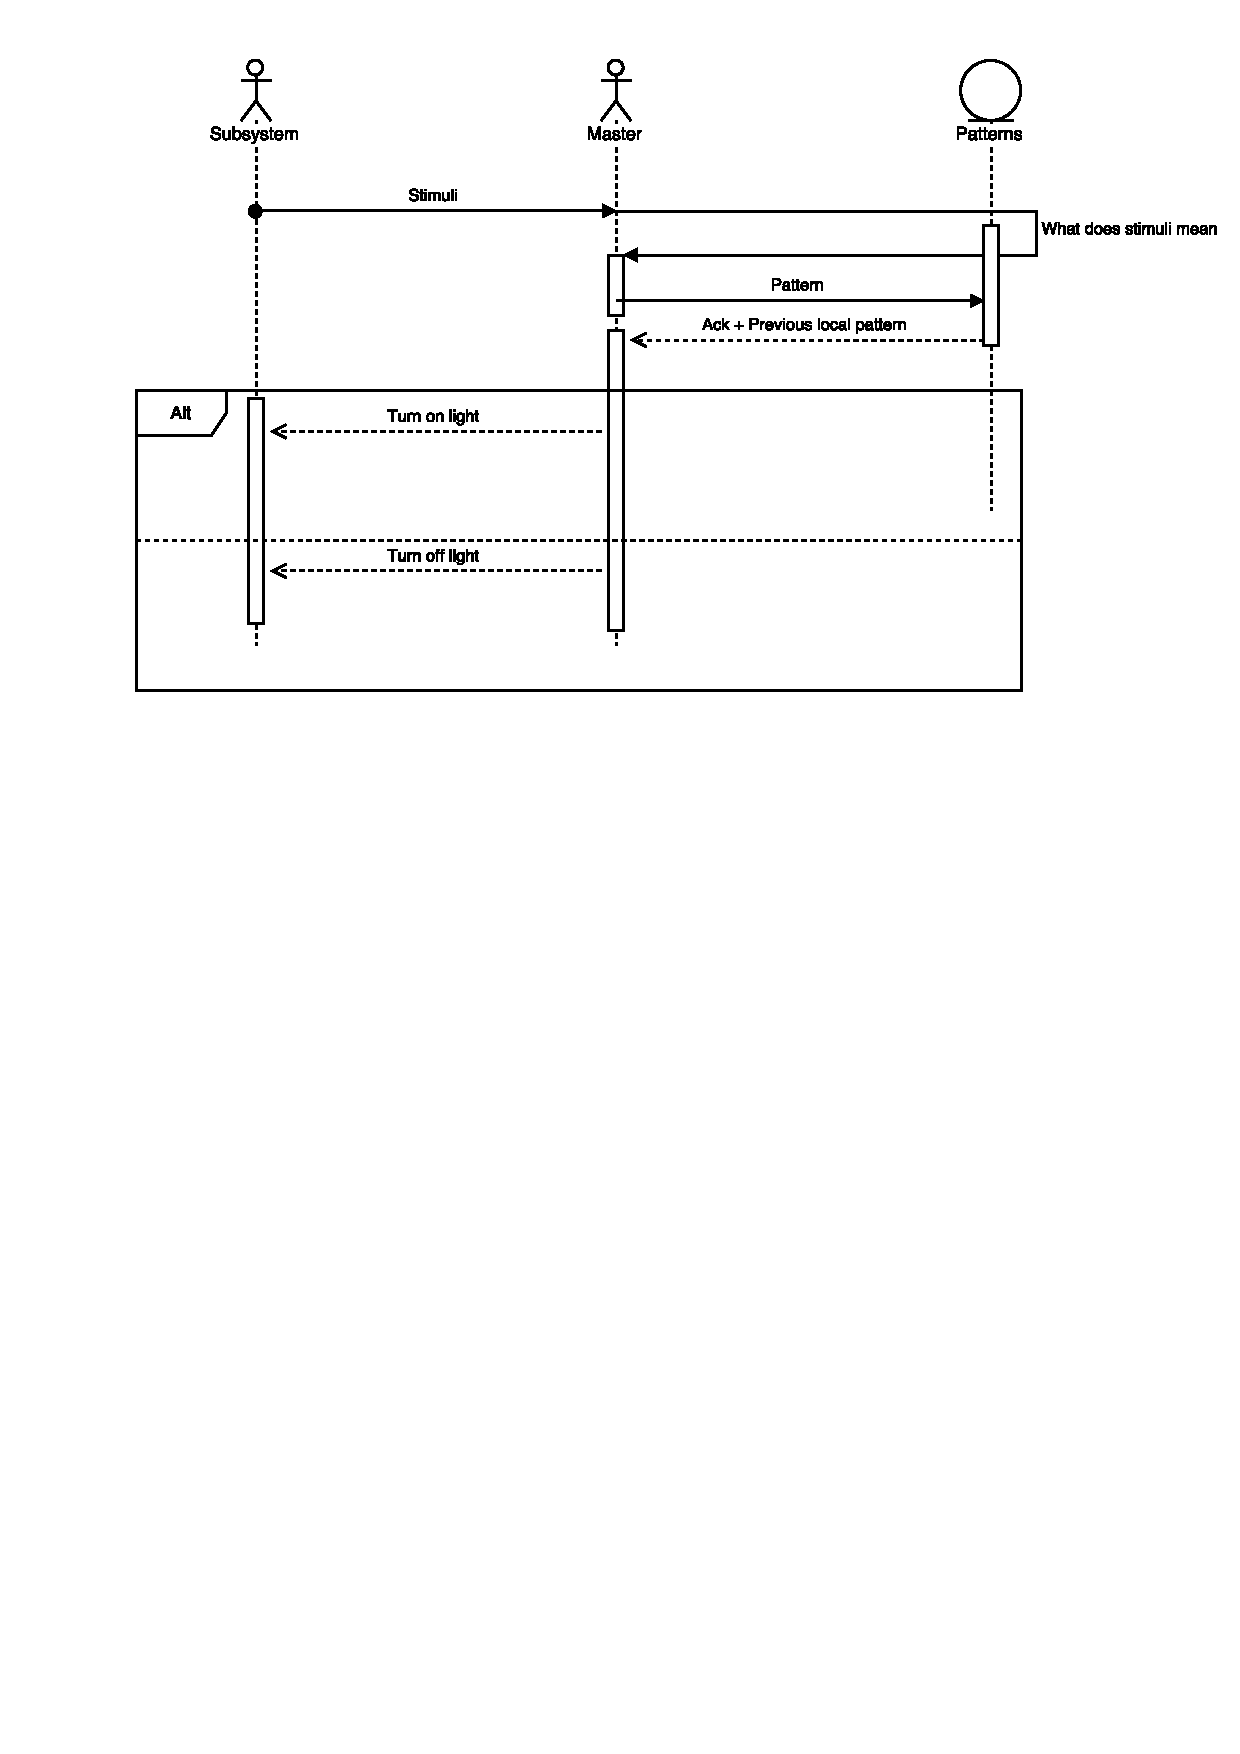
\includegraphics{Behaviour.pdf}
%    \end{adjustbox}
%    \caption{Behaviour diagram}
% \end{figure}


%mainfile: ../master.tex
\section{User scenarios}\label{sec:userscenarious}

This section will describe branches of possible narratives derived from the use cases, described in the \cref{sec:usecases}.

\textit{A user is reading a book, the light intensity of the sun is low now due the time of the day, and the user is having trouble reading. The system has learned that at this light intensity when the user is situated at the couch with tv not running, the user now wants the light to be on.}

\textit{A user is home alone in his/her living room. Now leaving a room to go the toilet but does not turn of the light in the living room, while on the toilet the user closes the door and does not observe the light in the living room being turned off by the system to conserve/save energy.}

\textit{A user just left home for a vacation, the user is leaves a few lights on due to stress, the system recognises this and switches the lights off. The user has not been home for 24 hours, the system now initiates in doing short cycles of simulating normal behaviour of the user in some rooms to seed the impression of someone being home, to proactively prevent attracting interest from any observing burglars.}

\textit{In a financial report an organisation recognises a substantial amount of funds is used on lighting the facility. The system generates a report on the lights around the facility, effective lighting hours. Which the supervisors can conclude on to argue were to invest on more energy efficient lighting. Further the system reports on broken or not functioning lighting.}


%Just for fun ? Many users is situated in the living room and the volume(db) of the stereo is really high, so users is shouting to hear each other and this occurs over prolonged duration, the system intellingently lowers the volume without the user noticing. And at 1am/pm(night) the user normally goes to sleep but not today, but because of neighbors the system lowers the volume further.



<<<<<<< HEAD
<<<<<<< HEAD
%mainfile: ../master.tex
\section{Use cases}\label{sec:usecases}

This section will describe ways of interacting with the prototypical system derived from the requirements.

<<<<<<< HEAD
<<<<<<< HEAD
<<<<<<< HEAD
=======
>>>>>>> 9c8f5030b9365c258596d255a2898784b52995cb
\begin{figure}
 \centering 
 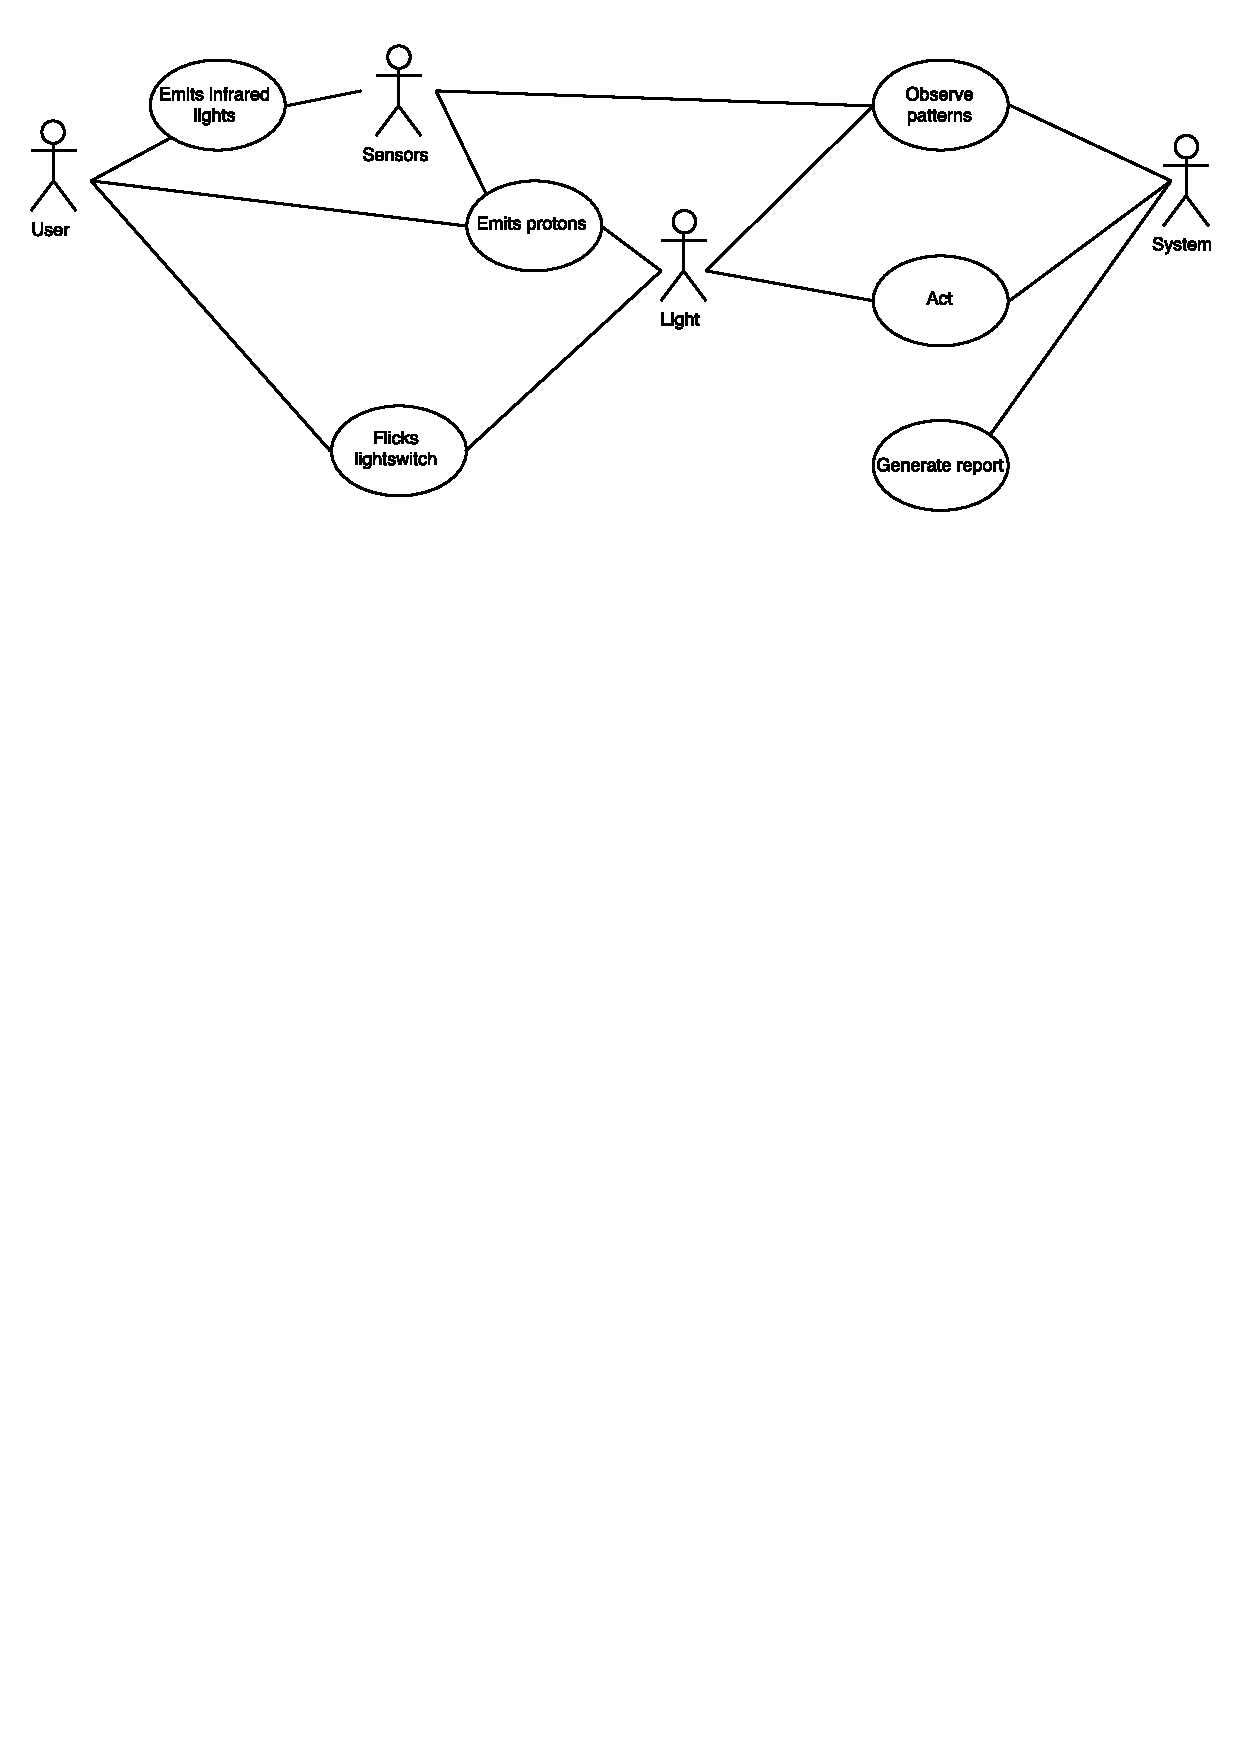
\includegraphics{Usecases.pdf}
 \caption{Rich picture of the problem domain}
\end{figure}
<<<<<<< HEAD
=======

>>>>>>> Specification refactor
=======
\begin{figure}
 \centering 
 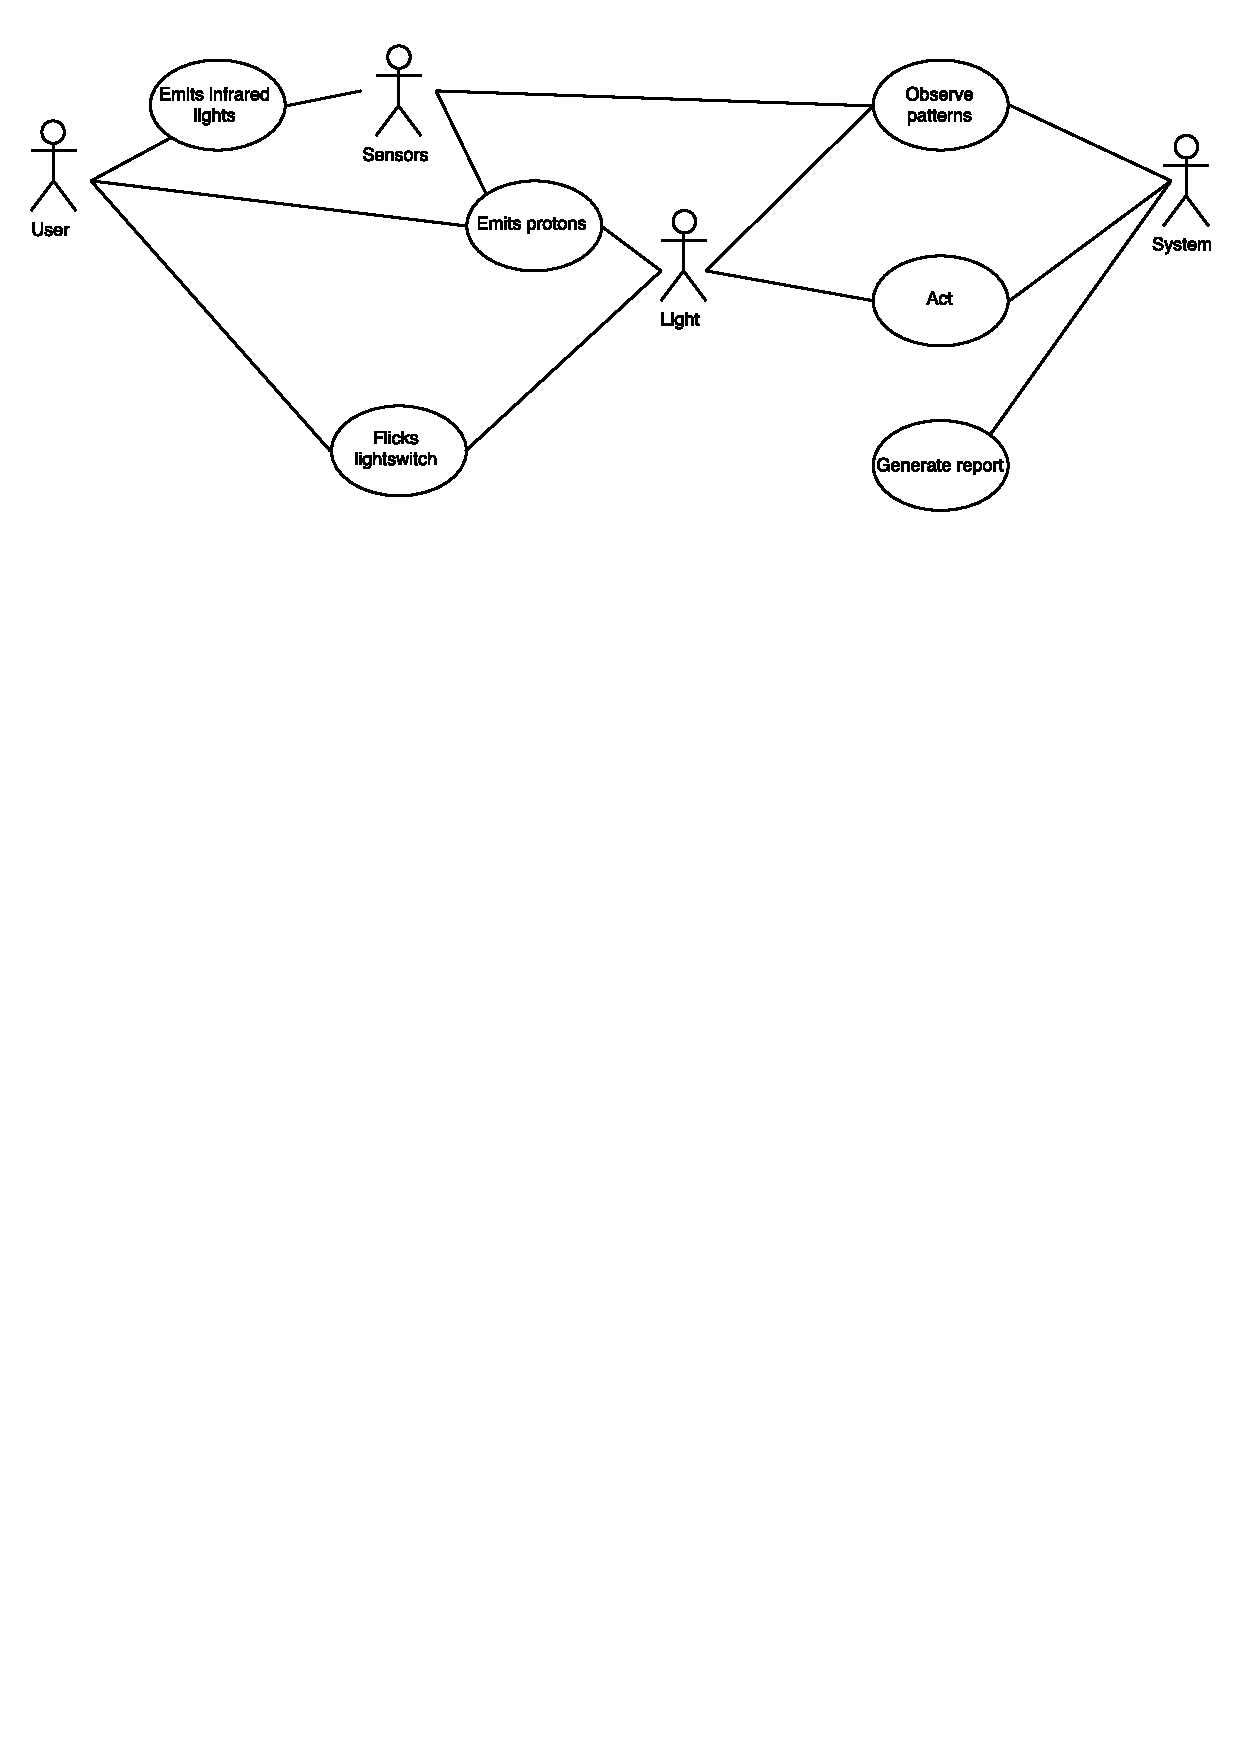
\includegraphics{Usecases.pdf}
\end{figure}
>>>>>>> More user scenarios
=======
>>>>>>> 9c8f5030b9365c258596d255a2898784b52995cb


%mainfile: ../master.tex
\section{structure}\label{sec:structure}

This section will describe what classes are associated to what classes. This will be useful for the designers and system when designing and reasoning about the knowledge base \cref{sec:KB}.





Elicited requirements: %Mangler argumentation
=======
\begin{itemize}
\item The light in a users home will be turned off when not in need for it
\item The light management invisible to the user, light is turned on before a user can observe this behaviour.
\item Will learn usage patterns of the user, turn on light at specific time of day or at a specific light intensity.
\end{itemize}

From the system definition and "rich picture" of the problem domain that the system will be operating, we can extract some classes, \quote{A description of a collection of objects with the same structure, behaviour and attributes}, as described in \cref{OOAD}. This classes will be beneficial when figuring out what we need to keep track of in the problem domain, or what is relevant in our model of the problem domain.

Classes:
\begin{itemize}
\item Person - The user of the system
\item Action - An action the system should recognise as feedback
\item Pattern - The usage patter of a user, what is typical behaviour
\item Mistake - System did something wrong by the user
\item Sensor - The observational member of the system
\item Switch - A feedback source
\item Lamp - The light source on which system action
\item Light intensity - Luminance
\item Room - What room is the user in
\item Premise - The user home enviroment
\item Time - At what time, a pattern property
\end{itemize}

\begin{table}[h!]
\centering
\begin{adjustbox}{max width=\textwidth}
\begin{tabular}{*{15}{|l}|}
    \hline
    \textbf{Event} & Person & Action & Pattern & Mistake & Sensor & Switch & Lamp & Light intensity & Room & Premise & Time \\
    \hline
    Entered home & \cmark & \cmark & \cmark & & \cmark & & \cmark & \cmark & \cmark & \cmark & \\
    \hline
    Left home & \cmark & \cmark & \cmark & & \cmark & & \cmark & & \cmark & \cmark & \\
    \hline
    Enter room & \cmark & \cmark & \cmark & & \cmark & & \cmark & \cmark & \cmark & & \\
    \hline
    Left room & \cmark & \cmark & \cmark & & \cmark & & \cmark & \cmark & \cmark & &\\
    \hline
    Flicked switch & \cmark & \cmark & \cmark & \cmark & \cmark & \cmark & \cmark & \cmark & \cmark & & \\
    \hline
    Outside/External light intensity down & \cmark & & & & \cmark & \cmark & \cmark & \cmark & \cmark & &\\
    \hline
    Outside/External light intensity up & \cmark & & & & \cmark & \cmark & \cmark & \cmark& \cmark & &\\
    \hline
    Person sleeping & \cmark & \cmark & \cmark & & \cmark & & \cmark & & \cmark & & \cmark\\
    \hline
\end{tabular}
\end{adjustbox}
  \caption{Test Table}
  \label{tab:label_test}
\end{table}
>>>>>>> merge

\begin{itemize}
\item The light in a users home will be turned off only when there is no need for it.
\item The user should be in doubt that the system will eventually turn off the light.
\item The should not be afraid that the system will suddenly turn off the light, whilst the user is need of it.
\item The light management should sought to be invisible to the user, light is turned on before a user can observe this behaviour.
\item Will learn usage patterns of the user, turn on light at specific time of day or at a specific light intensity.
\end{itemize}
=======
%mainfile: ../master.tex
\section{User scenarios}\label{sec:userscenarious}

This section will describe branches of possible narratives derived from the use cases, described in the \cref{sec:usecases}.

\textit{A user is reading a book, the light intensity of the sun is low now due the time of the day, and the user is having trouble reading. The system has learned that at this light intensity when the user is situated at the couch with tv not running, the user now wants the light to be on.}

\textit{A user is home alone in his/her living room. Now leaving a room to go the toilet but does not turn of the light in the living room, while on the toilet the user closes the door and does not observe the light in the living room being turned off by the system to conserve/save energy.}

\textit{A user just left home for a vacation, the user is leaves a few lights on due to stress, the system recognises this and switches the lights off. The user has not been home for 24 hours, the system now initiates in doing short cycles of simulating normal behaviour of the user in some rooms to seed the impression of someone being home, to proactively prevent attracting interest from any observing burglars.}

\textit{In a financial report an organisation recognises a substantial amount of funds is used on lighting the facility. The system generates a report on the lights around the facility, effective lighting hours. Which the supervisors can conclude on to argue were to invest on more energy efficient lighting. Further the system reports on broken or not functioning lighting.}


%Just for fun ? Many users is situated in the living room and the volume(db) of the stereo is really high, so users is shouting to hear each other and this occurs over prolonged duration, the system intellingently lowers the volume without the user noticing. And at 1am/pm(night) the user normally goes to sleep but not today, but because of neighbors the system lowers the volume further.


=======
%mainfile: ../master.tex
\section{User scenarios}\label{sec:userscenarious}

This section will describe branches of possible narratives derived from the use cases, described in the \cref{sec:usecases}.

\textit{A user is reading a book, the light intensity of the sun is low now due the time of the day, and the user is having trouble reading. The system has learned that at this light intensity when the user is situated at the couch with tv not running, the user now wants the light to be on.}

\textit{A user is home alone in his/her living room. Now leaving a room to go the toilet but does not turn of the light in the living room, while on the toilet the user closes the door and does not observe the light in the living room being turned off by the system to conserve/save energy.}

\textit{A user just left home for a vacation, the user is leaves a few lights on due to stress, the system recognises this and switches the lights off. The user has not been home for 24 hours, the system now initiates in doing short cycles of simulating normal behaviour of the user in some rooms to seed the impression of someone being home, to proactively prevent attracting interest from any observing burglars.}

\textit{In a financial report an organisation recognises a substantial amount of funds is used on lighting the facility. The system generates a report on the lights around the facility, effective lighting hours. Which the supervisors can conclude on to argue were to invest on more energy efficient lighting. Further the system reports on broken or not functioning lighting.}


%Just for fun ? Many users is situated in the living room and the volume(db) of the stereo is really high, so users is shouting to hear each other and this occurs over prolonged duration, the system intellingently lowers the volume without the user noticing. And at 1am/pm(night) the user normally goes to sleep but not today, but because of neighbors the system lowers the volume further.


>>>>>>> More user scenarios

%mainfile: ../master.tex
\section{Use cases}\label{sec:usecases}

This section will describe ways of interacting with the prototypical system derived from the requirements.

<<<<<<< HEAD
<<<<<<< HEAD
<<<<<<< HEAD
=======
>>>>>>> 9c8f5030b9365c258596d255a2898784b52995cb
\begin{figure}
 \centering 
 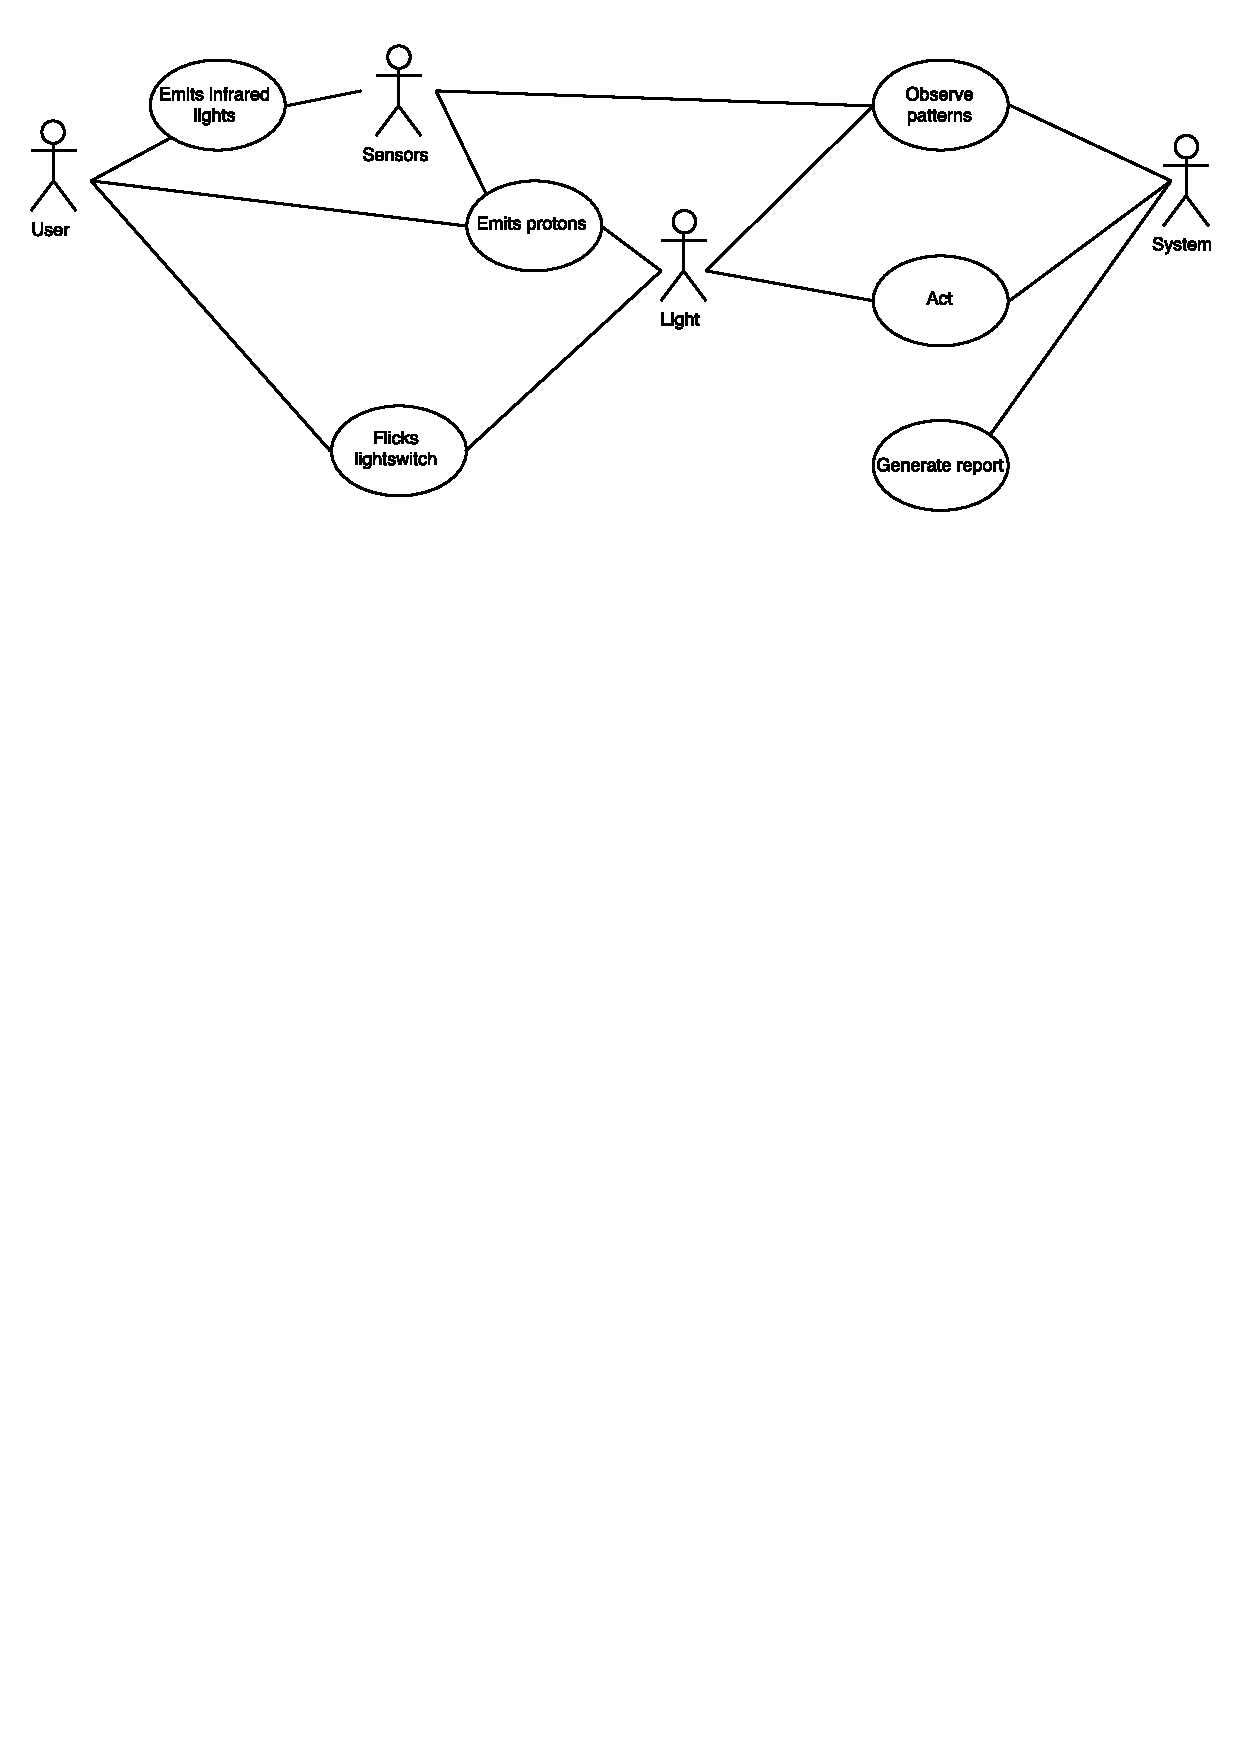
\includegraphics{Usecases.pdf}
 \caption{Rich picture of the problem domain}
\end{figure}
<<<<<<< HEAD
=======

>>>>>>> Specification refactor
=======
\begin{figure}
 \centering 
 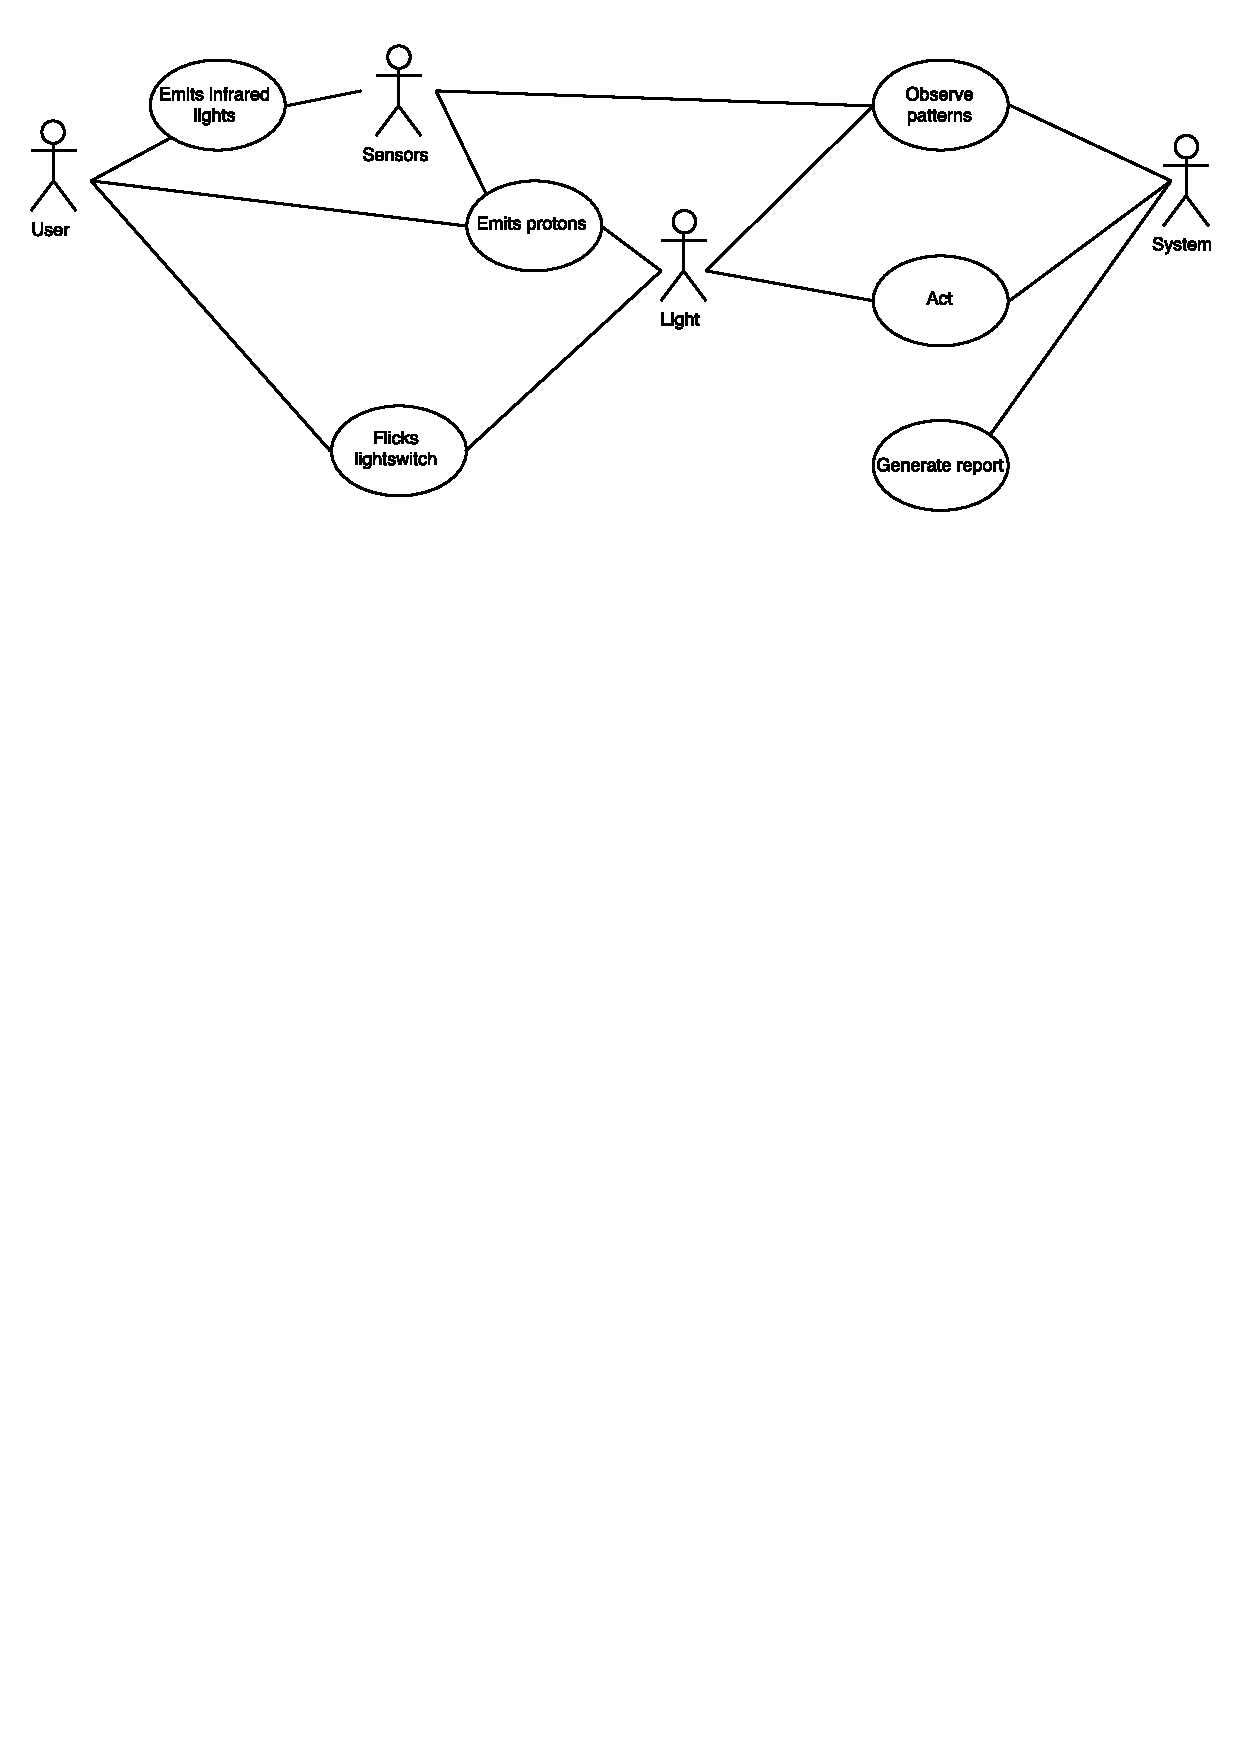
\includegraphics{Usecases.pdf}
\end{figure}
>>>>>>> More user scenarios
=======
>>>>>>> 9c8f5030b9365c258596d255a2898784b52995cb


>>>>>>> Specification refactor


\section{System Definition}

This section formally describes in which context the system is to be used, its
expected functions, the philosophy of the system, the conditions in which the
system is used, the technological aspect of the system, and the objects the
system should recognise and process.

\subsection{FACTOR}

The definition of the system can be decomposed into functionality, application
domain, conditions, technology, objects, and responsibility. This forms the
acronym FACTOR as introduced in \cite{mathiassen2001objektorienteret}.

\subsubsection{Functionality}

The system should be able to learn usage patterns of users, and autonomously
perform these actions.

\subsubsection{Application Domain}

The system should be used in homes where one or more users live. Each user may
have different usage patterns and sometimes irregular actions not part of their
daily routine.

\subsubsection{Conditions}

The system should adopt its actions to the wide-ranging usage patterns of a home
of multiple users.

\subsubsection{Technology}

The system should have small devices with accommodating sensors and actuators scattered strategically around the home.
These devices should be energy efficient in their use. Another computional
device should analyse sensor data collected by the small devices, and based on
the analysis, propose actions to be made autonomously by the system.

\subsubsection{Objects}

The system should recognise the users' patterns and their interaction with the
rest of the home.

\subsubsection{Responsibility}

The system should be as transparent to the user as possible to minimise friction
between the system and the user. This means that the user should not be
frustrated about the actions of the system. The system should be conservative
about its actions as to not perform actions the user would otherwise not have made.

\input{Analysis/ProblemFormulation.tex}